% Lecture Template for ME3023 -  Measurements in Mechanical Systems - Tennessee Technological University
% Spring 2020 - Summer 2020 - Fall 2020 - Spring 2021 - Summer 2021
% Tristan Hill, May 07, 2020 - June 12, 2020 - July 08, 2020 - Novemeber 02, 2020 - March 28, 2021 - May 25, 2021
% Module Name: - Introduction
% Topic 1 - General Measurement System

\documentclass[fleqn]{beamer} % for presentation (has nav buttons at bottom)

\usepackage{/home/thill/Documents/lectures/measurements_lectures/measurements_lectures}

\author{ME3023 - Measurements in Mechanical Systems} % original formatting from Mike Renfro, September 21, 2004

\newcommand{\TNUM}{1\hspace{2mm}} % Topic number 
\newcommand{\moduletitle}{Introduction}
\newcommand{\topictitle}{General Measurement System} 

\newcommand{\sectiontitleI}{Welcome Back!}
\newcommand{\sectiontitleII}{Definition of a Measurement}
\newcommand{\sectiontitleIII}{Measurement System Stages}
\newcommand{\sectiontitleIV}{Examples in Mechanical Engineering }

% custom box
\newsavebox{\mybox}

\title{Lecture Module - \moduletitle}

\date{Mechanical Engineering\vspc Tennessee Technological University}

\begin{document}

\lstset{language=MATLAB,basicstyle=\ttfamily\small,showstringspaces=false}

\frame{\titlepage \center\begin{framed}\Large \textbf{Topic \TNUM - \topictitle}\end{framed} \vspace{5mm}}

% Section 0: Outline
\begin{frame}

\large \textbf{Topic \TNUM - \topictitle} \vspace{3mm}\\

\begin{itemize}

	\item \hyperlink{sectionI}{\sectiontitleI} \vspc % Section I
	\item \hyperlink{sectionII}{\sectiontitleII} \vspc % Section II
	\item \hyperlink{sectionIII}{\sectiontitleIII} \vspc %Section III
	\item \hyperlink{sectionIV}{\sectiontitleIV} \vspc %Section IV

\end{itemize}

\end{frame}

% Section 1
\section{\sectiontitleI}

\begin{frame}[label=sectionI]
\frametitle{\sectiontitleI}
%\large{\it Welcome Back!\vspace{3mm}\\}

\begin{itemize}
\item Summer school is different but we will still cover the same material as we would in the regualar semester. \vspace{3mm}\\
\item These new outlines should help keep me/us on track.  \vspace{3mm}\\
\item The material will be organized in $\sim 10$ min videos, and you can watch them at anytime. \vspace{3mm}\\
\end{itemize}

\end{frame}

% Section 2
\section{\sectiontitleII}

\begin{frame}[label=sectionII]
\frametitle{\sectiontitleII}

\large{``A \hspcuu is an act of assigning a specific value to a physical variable.''} \vspc
{\tiny Text: Theory and Design of Mech. Meas.}

\end{frame}

% Section 3
\section{\sectiontitleIII}

\begin{frame}[label=sectionIII]
\frametitle{\sectiontitleIII}

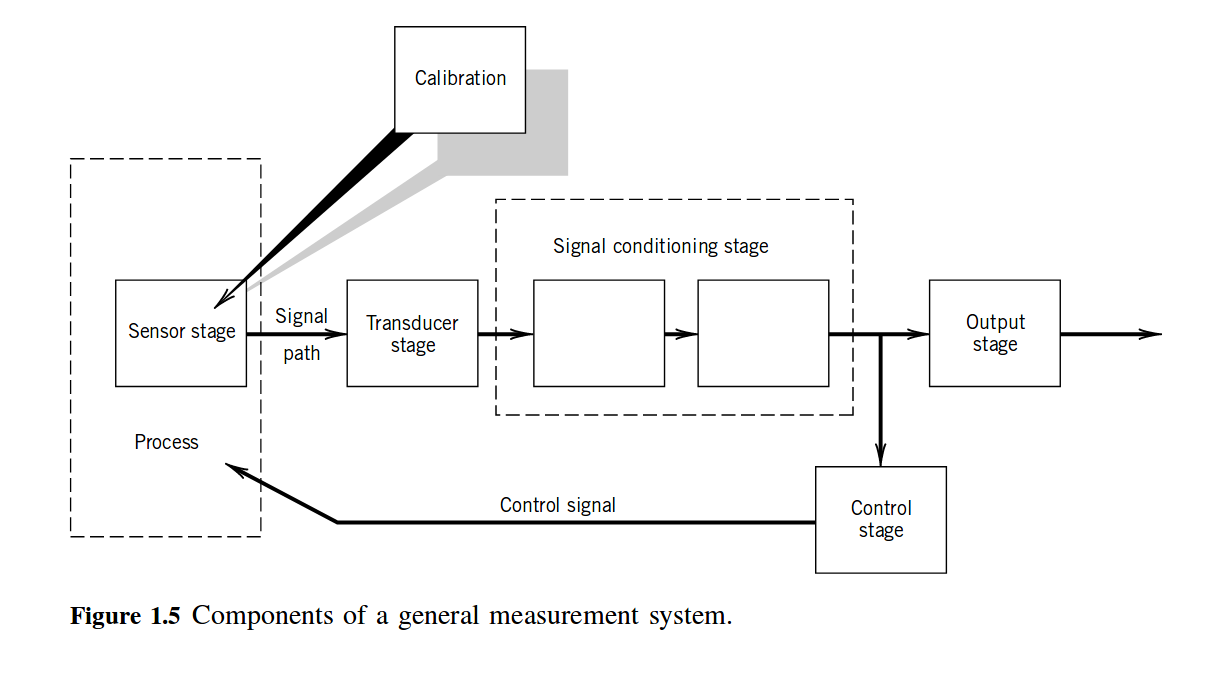
\includegraphics[scale=.3]{measurement_stages} \\
{\tiny Image: Theory and Design of Mech. Meas.}
\end{frame}

\begin{frame}
\frametitle{Sensor-Transducer Stage}
a \hspcuu, a physical element that employs some natural phenomenon... ...to sense the variable being measured
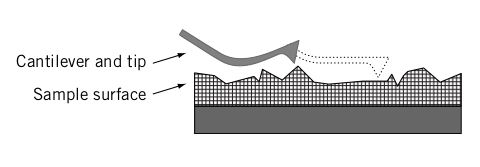
\includegraphics[scale=0.20]{sensor_stage.png}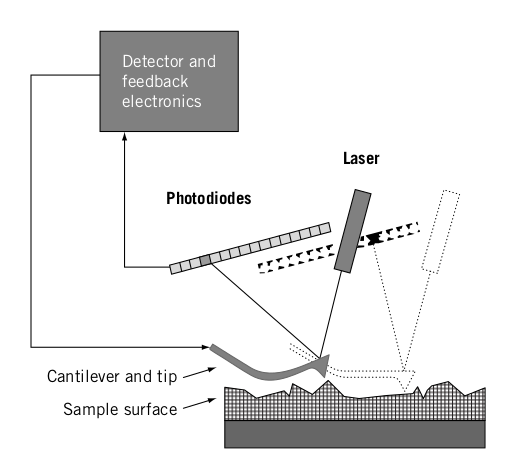
\includegraphics[scale=0.20]{sensor_transducer_stage}\\

A {\GR transducer} converts the sensed information into a \hspcuu \hspcc \hspcuu \\
{\tiny Text, Image: Theory and Design of Mech. Meas.}
\end{frame}

\frame{
\frametitle{Signal Conditioning Stage}

What is the the definition of {\BL signal}? \vspc

\begin{multicols}{2}
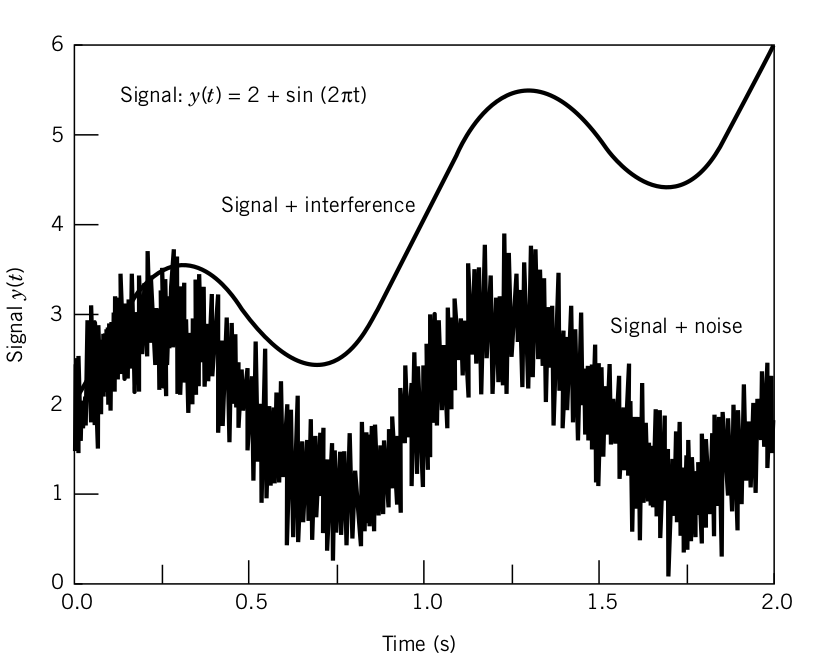
\includegraphics[scale=0.18]{signal_noise.png}

\begin{itemize}
\item Filtering
\item Amplification
\item Attenuation
\item Excitation 
\item Linearization
\item Electrical Isolation
\item Surge Protection
\end{itemize}

\end{multicols}

{\tiny Image: Theory and Design of Mech. Meas.}
}

\begin{frame}
\frametitle{Output Stage}
The \hspcuu \hspcc \hspcuu indicates or records the value measured. This might be a simple readout
display, a marked scale, or even a recording device such as a computer disk drive.

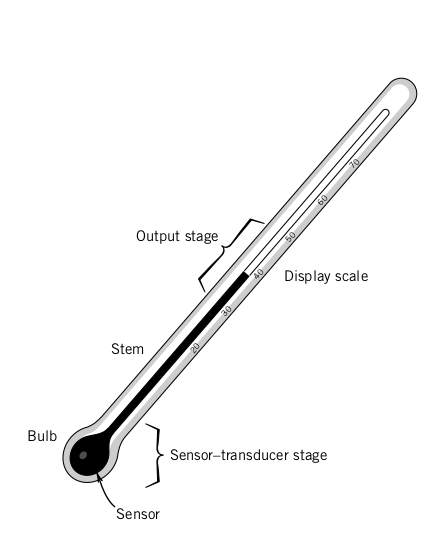
\includegraphics[scale=0.25]{bulb_thermometer.png} \hspace{10mm}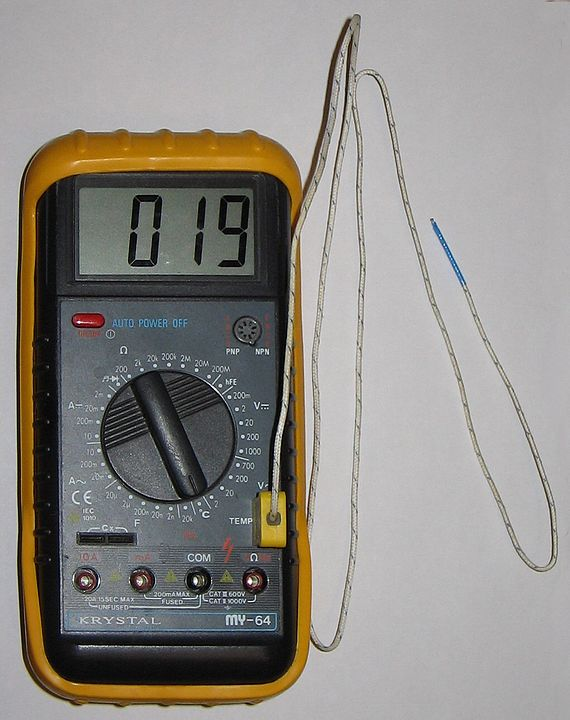
\includegraphics[scale=0.3]{thermocouple.jpg}

{\tiny Image: Theory and Design of Mech. Meas. \hspace{20mm} Image: \href{https://en.wikipedia.org/wiki/Thermocouple}{Wikipedia} }
\end{frame}

% Section 4
\section{\sectiontitleIV}

\begin{frame}[label=sectionIV]
\frametitle{\sectiontitleIV}

\begin{multicols}{2}
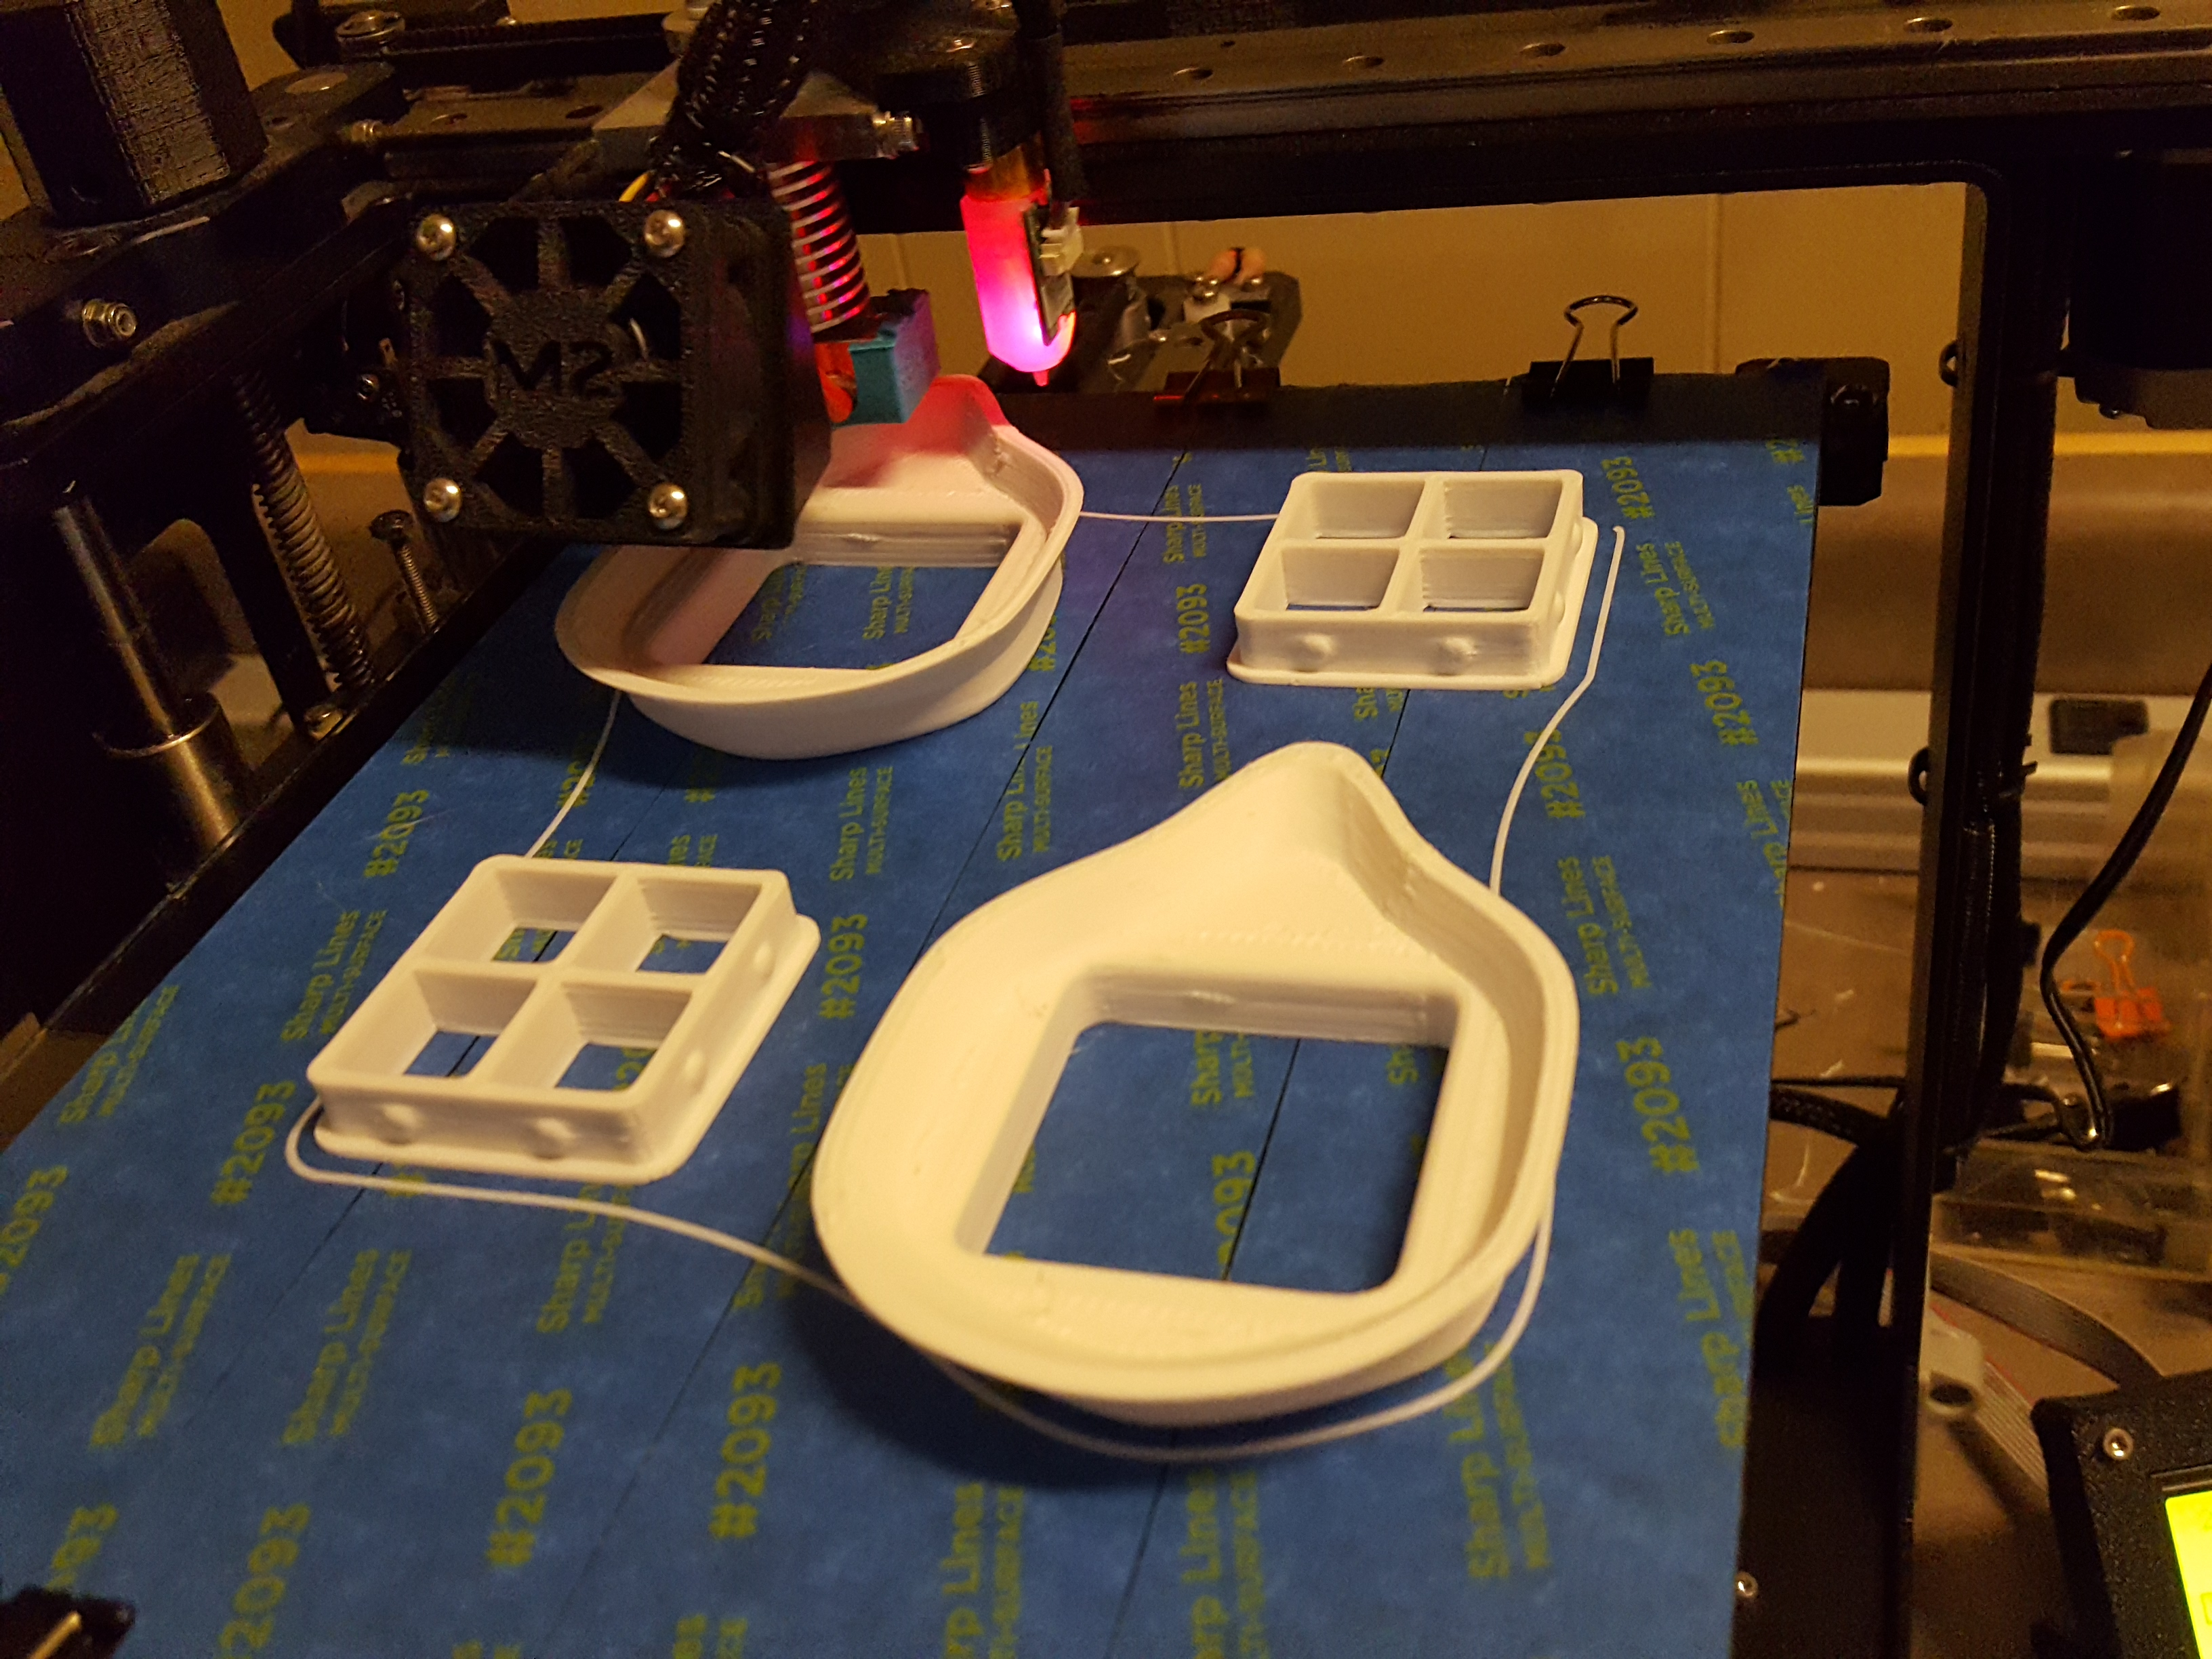
\includegraphics[scale=0.04]{makethemask.jpg}

\small
3D printers (FDM) use PLA, ABS, PETG and other plastics which absorb moisture from the air over time causing adverse affects on part quality. This is particularly a problem in humid climates such the southeastern USA.
\end{multicols}

{\tiny Image: T.Hill}

\end{frame}

\begin{frame}
\frametitle{Engineering Example}

\begin{multicols}{2}

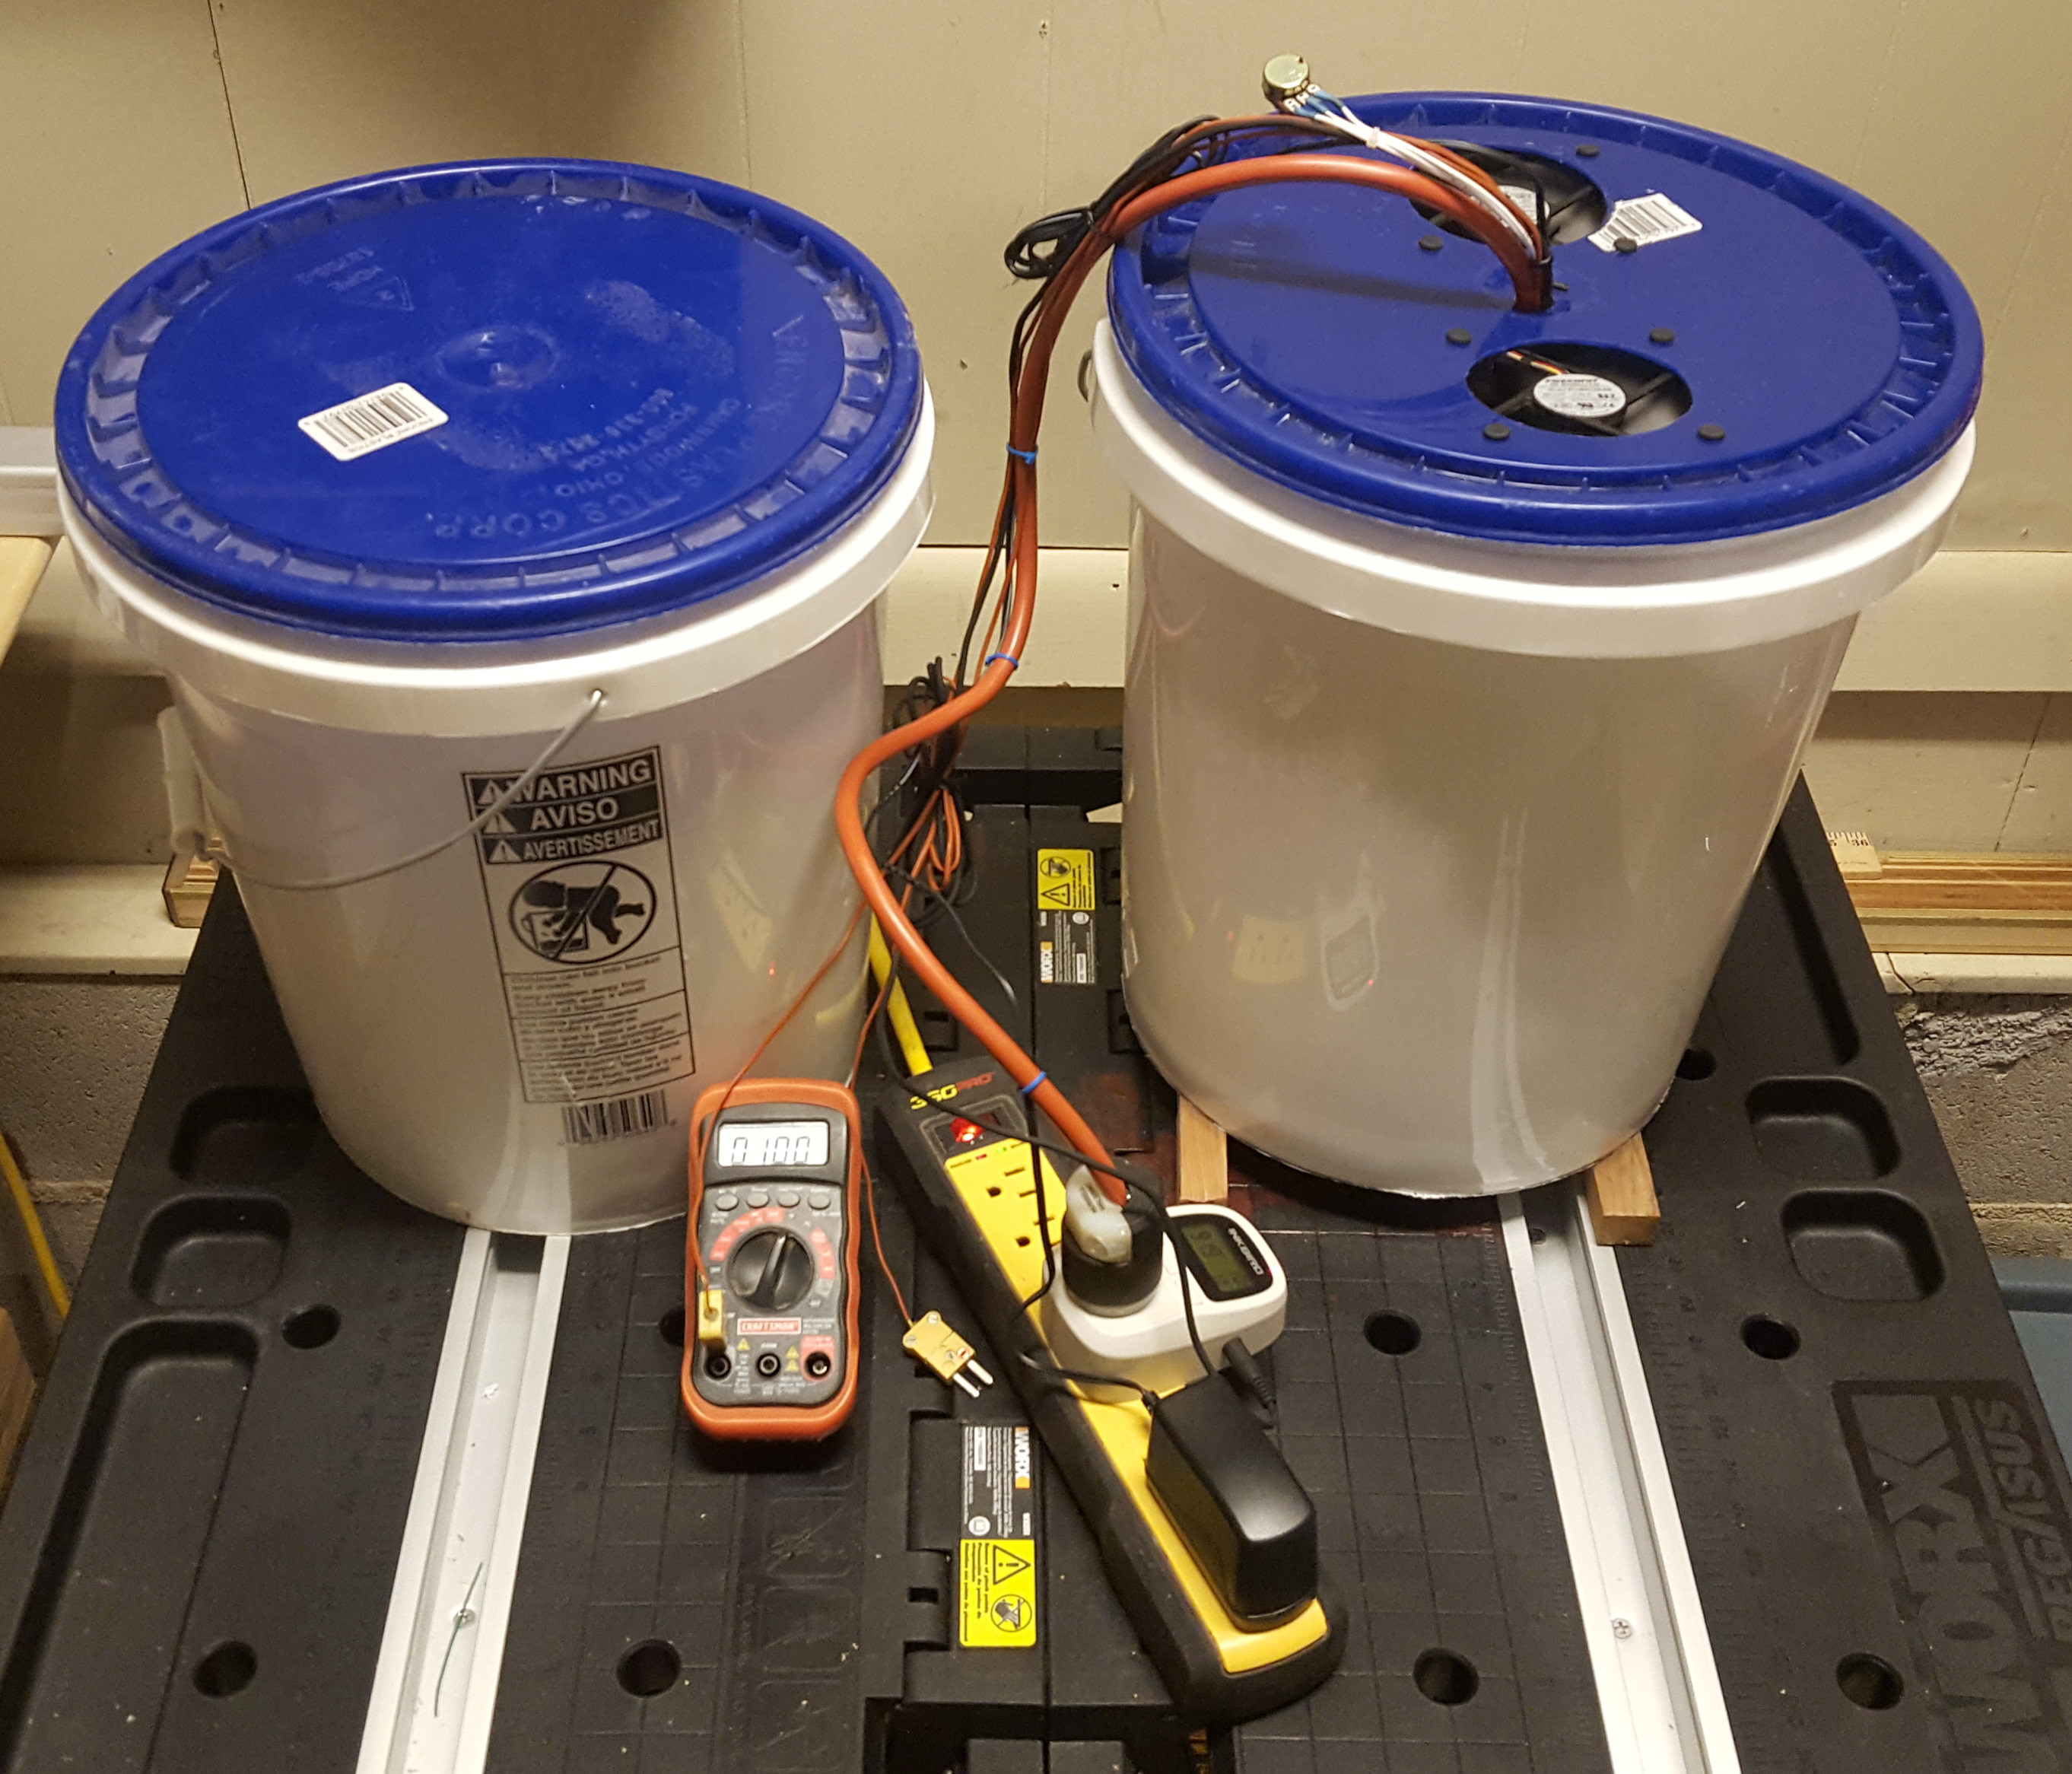
\includegraphics[scale=0.055]{filament_dryer_fig2.jpg}


\small
\vspace{10mm}Fortunately the {\it water-logged} plastic can be dehydrated for further use.\vspcc
Inspect the DIY filament dryer shown and Identify each of the following measurement stages.

\begin{itemize}
\item Sensor - Transducer
\item Signal Condtioning
\item Output Stage
\item Feedback Control ?
\end{itemize}

\end{multicols}

{\tiny Image: T.Hill}
\end{frame}

\end{document}





